\section{Szenariokonstruktion}
\label{constructions}
Als dritte und wichtigste Phase der Szenarioanalyse werden nun Szenarien aus den vorher definierten Einflussfaktoren erstellt. Hierfür bietet es sich an, die vorher ermittelten Entwicklunsausprägungen der einzelnen Schlüsselfaktoren auf Widerspruchsfreiheit zu überprüfen . Dafür wird eine Konsistenzanalyse genutzt \cite{spath}. Auf dessen Grundlage werden danach zukunftsfähige Anwendungsszenarien für die Skola GmbH erstellt.

\subsection{Konsistenzanalyse}

\begin{figure}
	\centering
	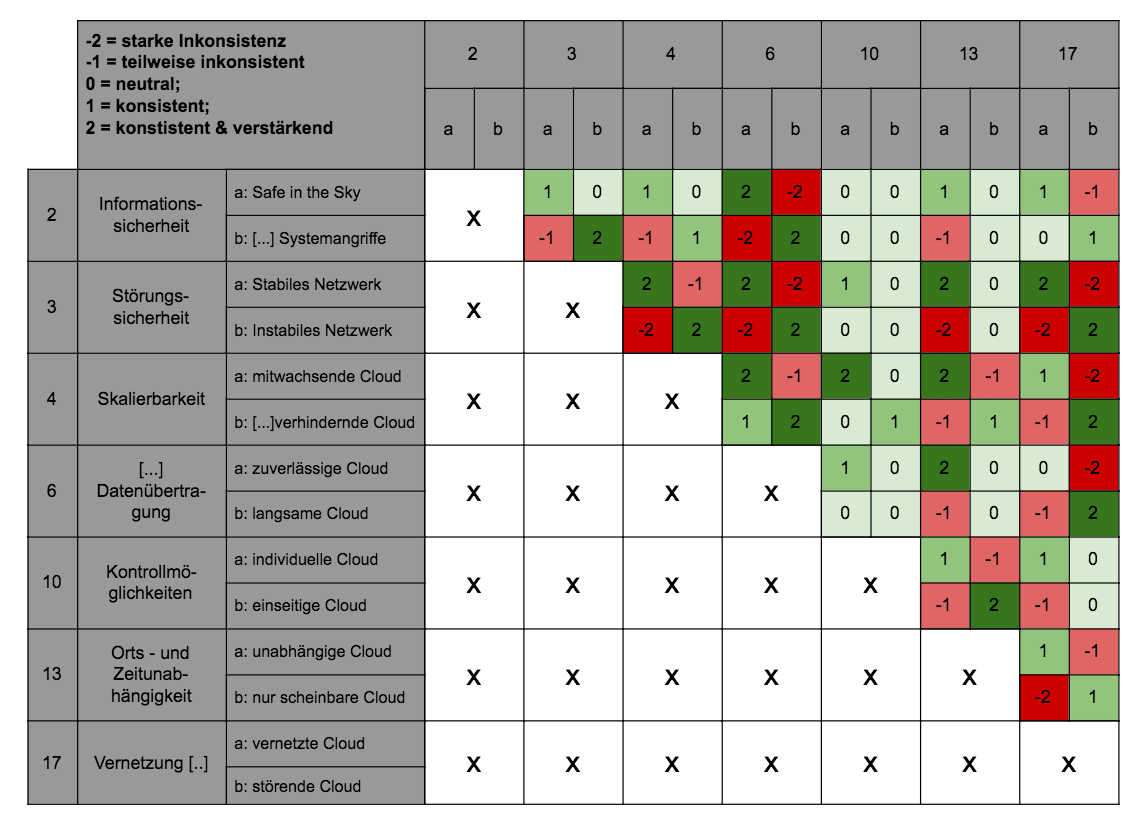
\includegraphics[width=\linewidth]{images/konsistenzanalyse}
	\caption[Caption for parameters]{Konsistenzanalyse}
	\label{fig:konsistenzanalyse}
\end{figure}

\todo[inline]{Auf Cloud Modelle Abschnitt 1 zurückgreifen!}
\subsection{Szenario 1}

\subsection{Szenario 2}

\subsection{Szenario 3}

